\documentclass[a4paper]{report}

\usepackage[round]{natbib}
\usepackage[nottoc,numbib]{tocbibind}
\usepackage{graphicx}
\usepackage[noline,noend,algoruled]{algorithm2e}
\usepackage{amsmath}
\usepackage{amssymb}
\usepackage{amsthm}
\usepackage[small]{caption}
\usepackage{subcaption}
\usepackage[table]{xcolor}

\newtheorem*{definition}{Definition}

\begin{document}

\title{Automatic Structural Inference of Binary Protocols}
\author{Fredrik Appelros \and Carl Ekerot}
\date{\today}
\maketitle

\begin{abstract}
An abstract is a brief summary of a research article, thesis, review,
conference proceeding or any in-depth analysis of a particular subject or
discipline, and is often used to help the reader quickly ascertain the paper's
purpose.
\end{abstract}

\tableofcontents

\chapter{Introduction}

\section{Background}
Communication protocols are the foundation of everyday networking tasks. Each
time a web page is served or an email is sent, a rigorous series of actions is
taken to ensure that the requested piece of information is relayed. The
information is packaged in a \emph{message} and both the syntax and the
semantics of these messages are defined by protocols.

Protocols may be open or closed in terms of available documentation. The reason
for them being closed might be that they are proprietary or simply because no
one invested in creating a documentation of the protocol in the first place.
Despite the lack of a documentation there still sometimes exists a need to
understand the inner workings of a certain protocol, e.g. when providing
interoperability between services. One infamous example of this is Microsoft's
proprietary SMB protocol which spawned the Samba project. This project was
created in an attempt to provide access to certain Windows services for
Unix-like operating systems. It did this through protocol analysis; a process
which took many years until most of the functionality of the SMB protocol had
been implemented.

Another area where the need for inferring the structures of closed protocols is
in \emph{deep packet inspection} (DPI). Messages sent over a network are
usually constructed hierarchically. At the bottom there is only raw binary data
and at the top there is the application data, e.g. an email or a video. There
in between exists several layers that contain metadata which is used to make
sure that the data reaches its target and that it does not get corrupted during
transmission. As a message is sent from one party to another it traverses a
series of nodes in the network. These nodes only needs to look at the lower
parts of the hierarchical structure of the message in order to relay it. If a
node wants to conduct DPI however, the higher levels of the hierarchy is looked
at as well.

There are many different reasons why one would want to perform DPI, one of
which is to provide \emph{quality of service} (QoS). QoS is needed in order to
gather statistics for Internet service providers that manage the networks. One
company that delivers QoS solutions is Procera Networks on whose behalf we are
writing this thesis.

\section{Related work}
Here is a discussion about related work. We talk about different methodologies
along with their respective advantages and disadvantages. As an example here
is a citation \citep{cui07}.

\chapter{Theory}

\section{Features}
In machine learning, a feature is a measurable property of the input data. An
example of a feature when working with images could be the intensity of light
for a certain pixel. Features do not need to directly correspond to a
physically measurable property however, instead they can be constructed by
transforming other features. These new high-level features can then be used
just like any other feature in order to simplify a complex problem.

One common type of complex problem is working with high dimensional data. There
are different ways to deal with such data; one of them being to use a solving
method that scales linearly. Another way is to reduce the dimensionality of the
problem itself.

\subsection{Principal component analysis}
One method to reduce the dimensionality of a problem is to use principal
component analysis (PCA). PCA transforms the input data into another dataset
where each dimension accounts for as much variance as possible while requiring
it to maintain orthogonality to the other dimensions. The new dataset can be
constructed to contain fewer dimensions than the original data and will then
capture as much variance as possible in the given number of dimensions. PCA can
be accomplished through singular value decomposition of a matrix.

\section{Simple linear regression}
In statistics, a response variable $Y_i$ that is linearly dependent on an
explanatory variable $X_i$ can be modeled with a simple linear regression
model. The relationship between the two variables are then

\begin{equation}
    Y_i = \alpha + \beta X_i + \varepsilon_i
    \label{eq:slr}
\end{equation}

where $\alpha$ and $\beta$ are the \emph{regression coefficients} and
$\varepsilon_i$ is the error term. Given a set of data
$\displaystyle \{Y_i, X_i\}_1^n$ the regression coefficients can be estimated
through linear regression. This process is often called fitting as it can be
seen as trying to find the model with the best fit for the data. There are
different methods to do this as there is no consistent measure for what is the
best fit.

\subsection{Ordinary least squares}
Ordinary least squares (OLS) is a method for estimating the regression
coefficients in equation~\ref{eq:slr}. It does this by minimizing the sum of
squared residuals of the simple linear regression model. This can be formulated
as minimizing the following cost function.

\begin{equation}
    C(\alpha, \beta) = \sum_{i=1}^n(Y_i - \alpha - \beta X_i)^2
\end{equation}

The result of this is a model that minimizes the residuals globally across all
samples. This intrinsically makes the method \emph{non-robust}, i.e. sensitive
to outliers.

{
    \fontsize{10}{12}
    \selectfont
    \begin{algorithm}[t]
        \DontPrintSemicolon
        \BlankLine
        \KwIn{$D$, $M$, $n$, $\delta$, $\gamma$, $k$}
        \KwOut{$P_b$}
        \BlankLine
        $P_b \gets \varnothing$\;
        $\varepsilon_b \gets \infty$\;
        \For{$k$}{
            $I \gets n$ number of randomly chosen samples\;
            fit $M$ to $I$\;
            $I_m \gets$ samples where distance from $M \leq \delta$\;
            $I \gets I \cup I_m$\;
            \If{$|I| \geq \gamma$}{
                fit $M$ to $I$\;
                $\varepsilon \gets$ deviation from $M$ for all $I$\;
                \If{$\varepsilon < \varepsilon_b$}{
                    $P_b \gets$ parameters in $M$\;
                    $\varepsilon_b \gets \varepsilon$\;
                }
            }
        }
        \Return{$P_b$}
        \BlankLine
        \caption{RANSAC}
        \label{alg:ransac}
    \end{algorithm}
}

\subsection{RANSAC}
Random Sample Consensus (RANSAC) \citep{fischler81} is a \emph{robust} method
for fitting a dataset to a model and was originally intended for image
analysis. The robustness of the method allows it to avoid the influence of
outliers in the model. Given a dataset $D$, a model $M$, a set of inliers $I$
and two confidence parameters, $\delta$ and $\gamma$, it works the following
way:

\begin{enumerate}
    \item Fit $M$ to $I$
    \item Find the samples that are within $\delta$ distance from $M$ and add
        those samples to $I$
    \item Continue if $|I|$ is at least $\gamma$
    \item Fit $M$ to $I$
    \item Evaluate $M$ from the residual of $I$
\end{enumerate}

One problem with this approach is that an initial set of inliers is required.
In most cases this is not available so we need to guess which samples might be
inliers. A simple solution to this is to take $n$ random samples and assume
that they are inliers. This only works if the assumption is actually true and
thus the resulting algorithm will be \emph{non-deterministic}, meaning that it
only produces a good fit with a certain probability. The algorithm is normally
run $k$ number of iterations until the probability of success is sufficiently
large. Pseudocode for RANSAC can be seen in algorithm~\ref{alg:ransac}.

The model that RANSAC operates on can be any kind of mathematical model, 
therefore when handling two-dimensional linear data the simple linear
regression model given in equation~\ref{eq:slr} can be used. This gives us a
method that solves the problem of simple linear regression but that is also
insensitive to outliers. A comparison between OLS and RANSAC on a dataset where
some samples have been replaced by random noise can be seen in
figure~\ref{fig:ransac}.

\begin{figure}[t]
    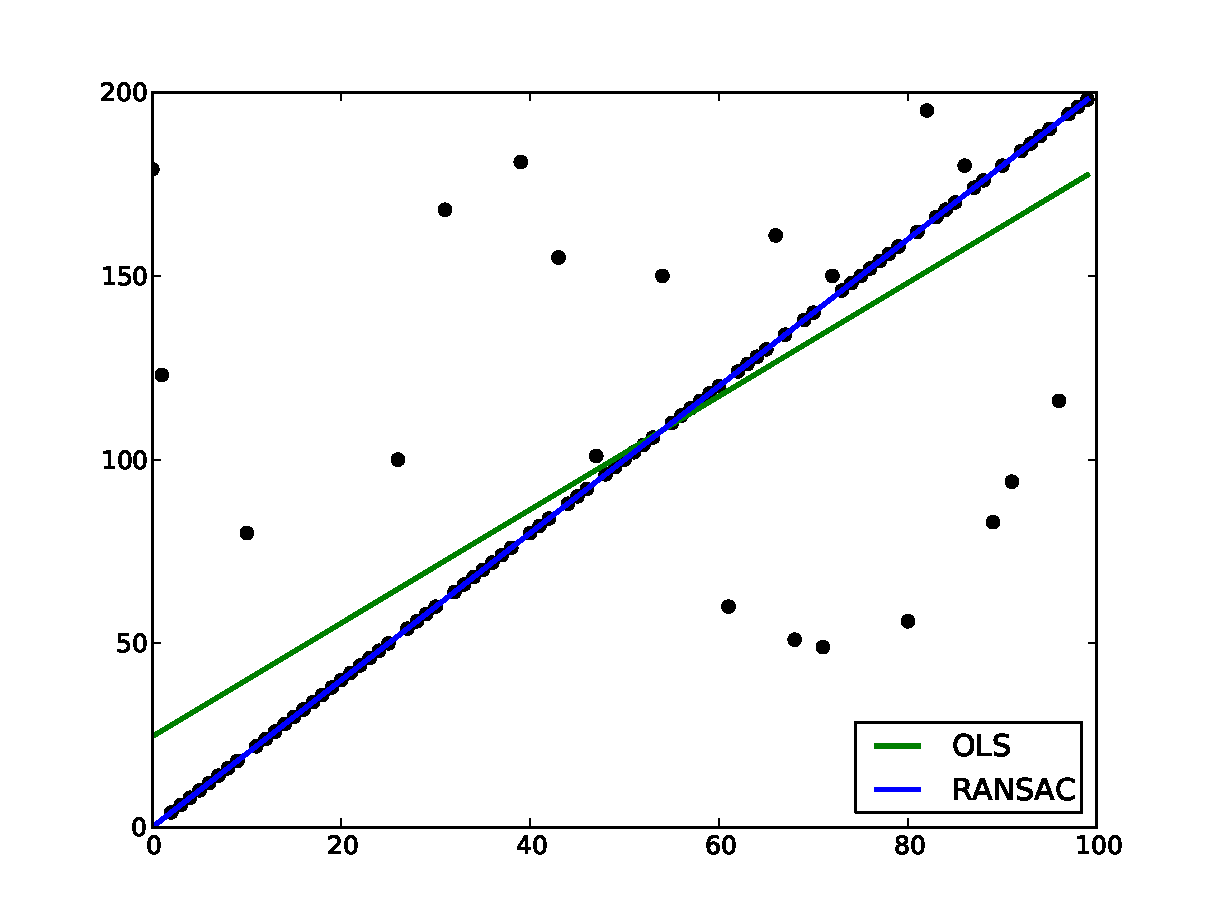
\includegraphics[width=\linewidth]{ransac}
    \caption{A comparison between OLS and RANSAC on a dataset containing
    outliers.}
    \label{fig:ransac}
\end{figure}

\section{Clustering}
A clustering is a grouping of samples based on similarity with respect to their
features. The features are predefined to represent distinct properties of the
samples. Similarities between samples are normally represented as distances in
an $n$-dimensional space, where $n$ is the number of features. Distances may be
calculated using any suitable norm.

In cluster analysis, the goal is normally to find a clustering from a
set of samples such that the membership of a cluster represents some true
relationship. In some clustering algorithms such as K-means \citep{macqueen67},
the number of clusters are predefined. When the number of clusters are unknown,
other algorithms such as DBSCAN, OPTICS and hierarchical clustering methods may
be used.

The clustering algorithm we use in our method is OPTICS, which is based on
DBSCAN. In the rest of this section we will explain these algorithms and
provide examples based on protocol data.

\subsection{DBSCAN}
DBSCAN is a \emph{density-based} clustering algorithm, as opposed to
partitioning clustering algorithms such as K-means. Density-based clustering 
algorithms provides the benefit of not having to provide an estimated number 
of clusters as a parameter to the algorithm.

DBSCAN was first presented by \citet{ester96}. The algorithm takes a set of 
samples $D$ and two parameters, $MinPts$ and $\varepsilon$. $MinPts$ decides
how many samples that are needed in order to form a cluster.

The densities are defined by the distances between a set of points.
The algorithm introduces the definition \emph{$\varepsilon$-neighborhood}
$N_{\varepsilon}(p)$ for a point $p$. The samples which are in 
$N_{\varepsilon}(p)$ are given by the following condition:

\begin{equation}
    N_{\varepsilon}(p) = \{ q \in D ~|~ dist(p,q) < \varepsilon  \}
    \label{eq:eps}
\end{equation}

The samples in $N_{\varepsilon}(p)$ are defined as \emph{directly density-
reachable} from $p$. Given that $|N_{\varepsilon}(p)| \ge MinPts$, the samples
in $N_{\varepsilon}(p)$ forms a cluster, and $p$ is a \emph{core point}. 

A cluster is not limited to containing samples which are direcly
density-reachable. The DBSCAN algorithm also defines that samples which are
not directly density-reachable may be \emph{density-reachable}.
A sample $q$ is density-reachable from a sample $p$ if there is a set of samples
$S = \{s_1, .., s_n\}$ where $p = s_1$, $q = s_n$ and $s_{i+1}$ is directly
density-reachable from $s_i$ for $0 < i < n$.

Since the density-reachable relationship is not symmetric, a looser
relationship is introduced: \emph{density-connected}. Two samples $p$ and
$q$ are density-connected if there exists a third point $o$ from which both
$p$ and $q$ are density-reachable. The density-connected relationship
is symmetric.

With these relationships, the algorithm defines cluster membership as
follows:

\begin{definition}
    The following conditions needs to be satisfied for a point $q$ to be a
    member of a cluster $C$, given that there is a sample $p \in C$:
    \begin{enumerate}
        \item $q$ is density-reachable from $p$
        \item $q$ is density-connected to $p$
    \end{enumerate}
\end{definition}

One of the drawbacks of DBSCAN is that it can only find clusters with a density
higher than the density decided by the $\varepsilon$-parameter. It is also hard
to estimate the $\varepsilon$ and $MinPts$-parameters for an unknown dataset.
This makes DBSCAN suitable for classifying data into known classes, but not as
suitable for finding underlying structures in entirely unknown datasets. In
figure~\ref{fig:dbscan} is an example of DBSCAN running on 5000 packets of DNS
data. The parameters are manually selected to $\varepsilon = 0.085$ and
$MinPts = 200$.

\begin{figure}[h]
    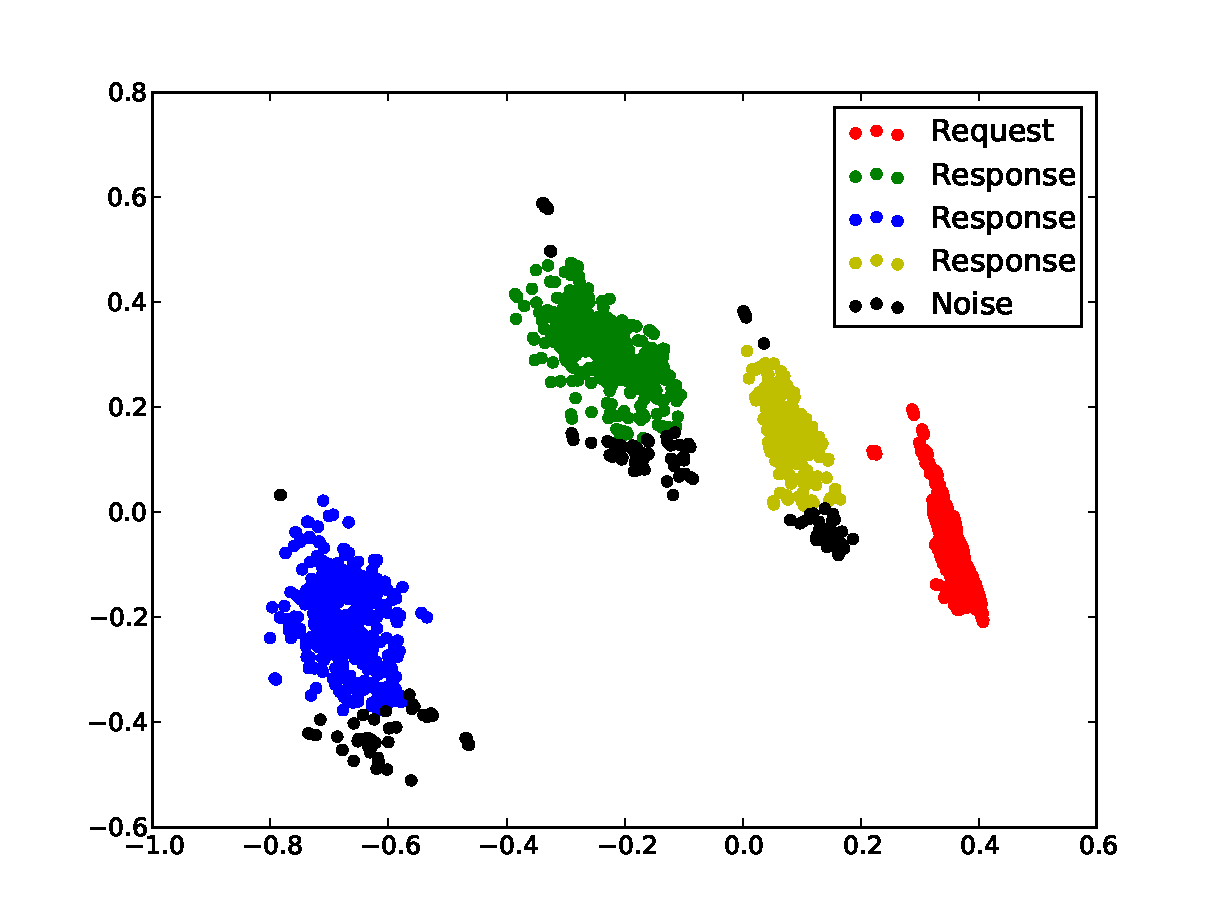
\includegraphics[width=\linewidth]{dbscan_dns}
    \caption{An example of clustering with DBSCAN running on samples generated
    from 5000 packets of DNS data.}
    \label{fig:dbscan}
\end{figure}

\subsection{OPTICS}
Addressing the difficulties in selecting parameters for DBSCAN,
\citet{ankerst99} introduced the OPTICS algorithm, which is an extension of
the concepts introduced in DBSCAN. OPTICS uses the definitions
\emph{directly density-reachable}, \emph{density-reachable} and
\emph{density-connected} which were described in the DBSCAN algorithm, but
eliminates the need for an explicit $\varepsilon$ parameter. Instead the
$\varepsilon$ parameter is interpreted as the largest distance to consider
when clustering. The results is an algorithm which is less sensitive to
user-specified parameters, and is able to find clusters with varying densities.

One important aspect of OPTICS is that it does not generate actual clusters.
Instead, it generates an \emph{ordering} of samples and a set of corresponding
\emph{reachability-distances} which reveals density-based structure in the
input data. The OPTICS algorithm extends DBSCAN with the definitions
\emph{core-distance} and \emph{reachability-distance}.
\\[0.5cm]
Core-distance is a measurement of the distance $\varepsilon$ which is required
for a sample $p$ to be a core point. That is, a core distance is the distance
$\varepsilon$ which satisfies $|N_{\varepsilon}(p)| = MinPts$.

\begin{definition}
    The core-distance for a sample $p$ is defined as:
\[
    \begin{cases}
        \text{UNDEFINED}, & \text{if $|N_{\varepsilon}(p)| < MinPts$}\\
        \text{Min $\varepsilon$ which satisfies  $|N_{\varepsilon}(p)| = MinPts$}(p), & \text{otherwise}
    \end{cases}
\]
\end{definition}

The core-distance is $UNDEFINED$ when an upper limit on $\varepsilon$ is
given as a parameter to the algorithm. This parameter is not required,
although it has an impact on the runtime of the algorithm.
\\[0.5cm]
The reachability-distance of a sample $p$ is the smallest distance which is
needed for $p$ to be directly density-reachable to a core point $q$ for some
$\varepsilon$. 

\begin{definition}
    The reachability-distance of a sample $p$ with respect to some sample $q$
    is defined as:
\[
    \begin{cases}
        \text{UNDEFINED}, & \text{if $|N_{\varepsilon}(q)| < MinPts$}\\
        \text{max(core-distance($q$), distance($q$, $p$))}, & \text{otherwise}
    \end{cases}
\]
    where distance($q$, $p$) is the smallest $\varepsilon$ for which $q$ is
    density-reachable from $p$.
\end{definition}

From the ordering and reachability-distances, the cluster structure may be
visualized in a \emph{reachability-plot}. The reachability-plot provides an
overview of the output from OPTICS as a barplot where the bars represent
reachability-distances in the ordering generated by OPTICS.

An example of a reachability plot generated from 5000 DHCP-packets with 
$MinPts = 500$ is shown in figure~\ref{fig:rplot}. Valleys in the
reachability-plot represents samples which are close to each other. Spikes
represents a large difference in distance between the samples to the left and
right of the spike.

\begin{figure}[t]
    \centering
    \begin{subfigure}[b]{0.48\linewidth}
        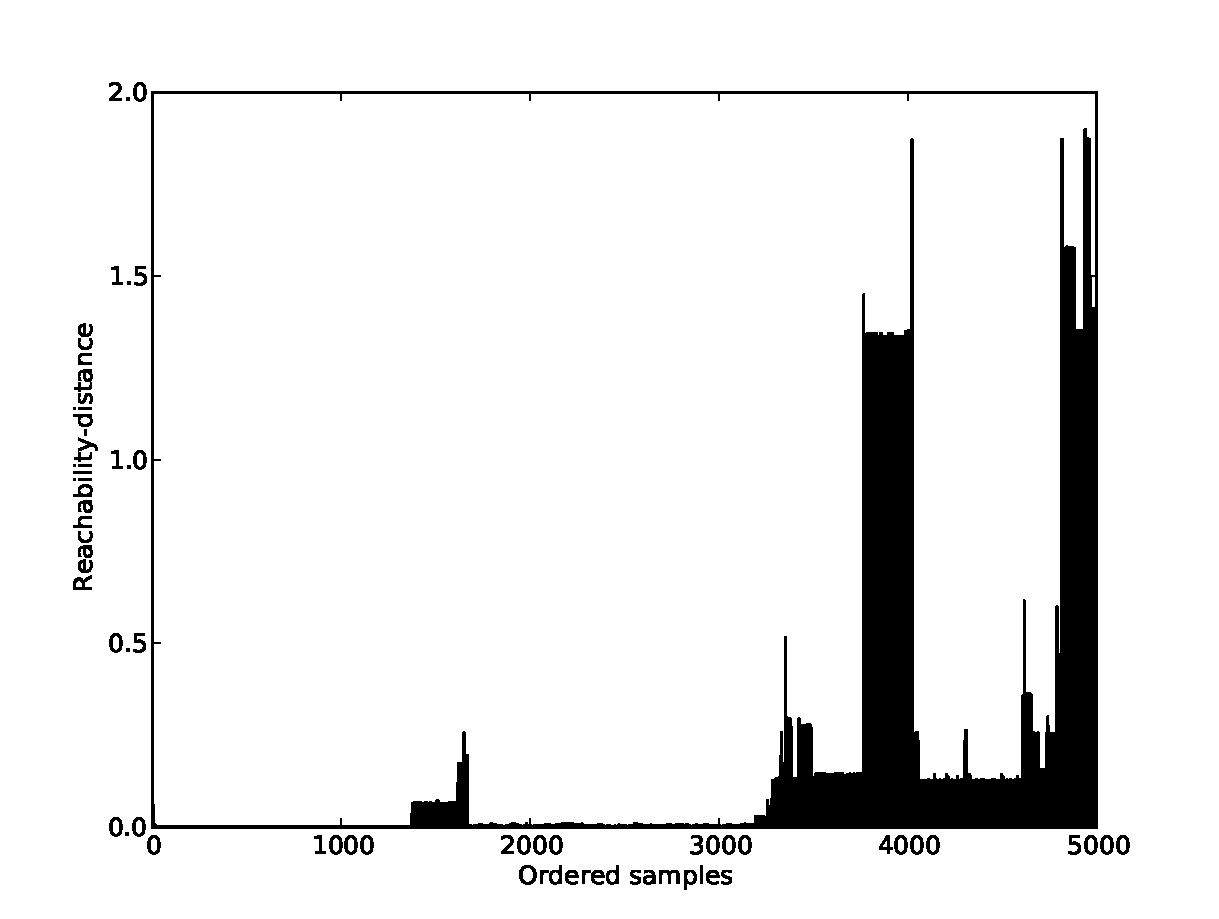
\includegraphics[width=\linewidth]{rplot_dhcp}
        \caption{Reachability-plot.}
        \label{fig:rplot}
    \end{subfigure}
    %\quad
    \begin{subfigure}[b]{0.48\linewidth}
        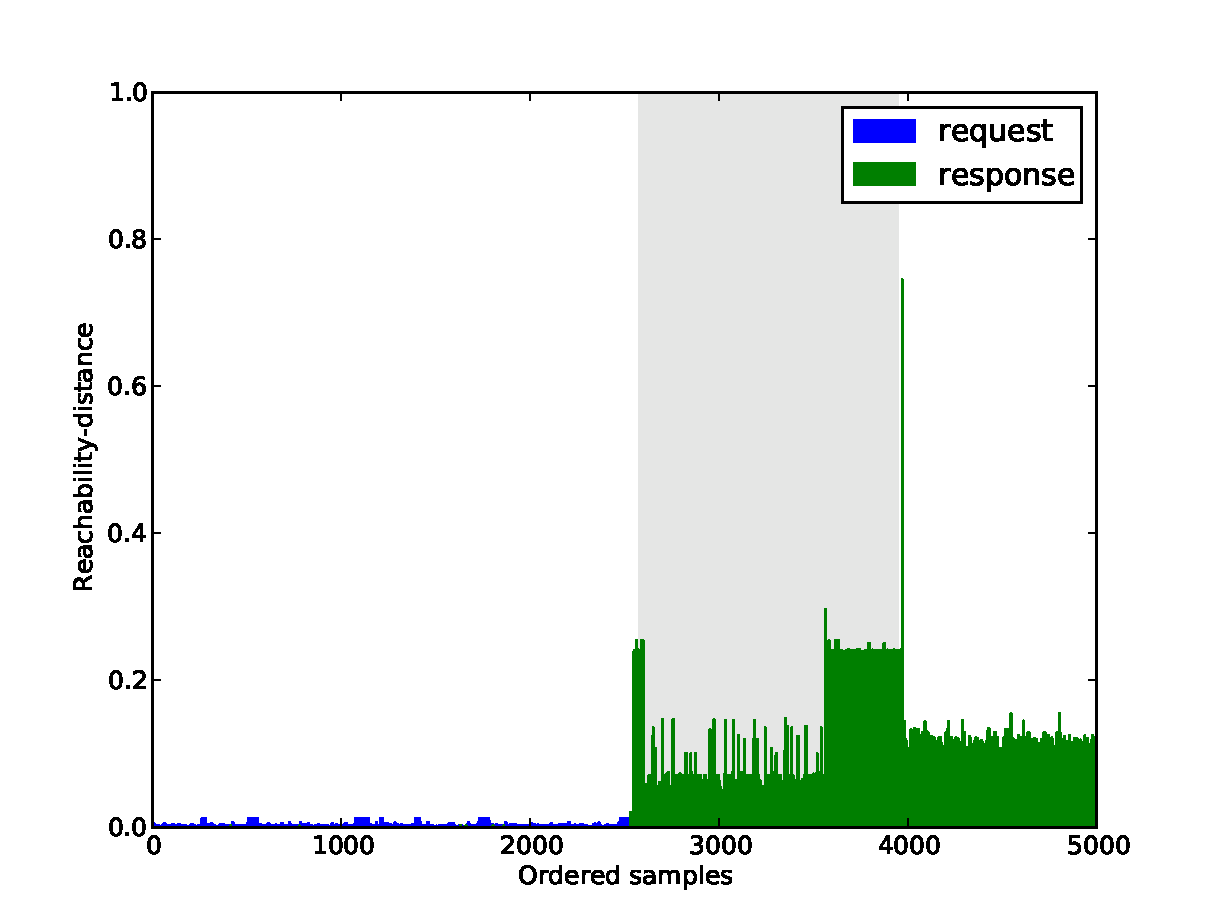
\includegraphics[width=\linewidth]{hierextr}
        \caption{Hierarchical extraction.}
        \label{fig:hierextr}
    \end{subfigure}
    \caption{caption}
    \label{fig:rplots}
\end{figure}

\subsubsection{Algorithm}
{
    \fontsize{10}{12}
    \selectfont
    \begin{algorithm}[H]
        \DontPrintSemicolon
        \BlankLine
        \KwIn{$D$, $MinPts$, $\varepsilon$}
        \KwOut{$ordering$, $reachability$-$distances$}
        \BlankLine

        $reachability$-$distances \gets \varnothing$\;
        $ordering \gets \varnothing$\;
        $seeds \gets 0,1,...,|D|$\;
        $i \gets 0$\;

        \While{$|seeds| > 1$} {
            $p \gets seeds.get(i)$\;
            $seeds.remove(i)$\;
            $ordering.add(p)$\;

            \If{$core$-$distance_{\varepsilon, MinPts}(p) \le \varepsilon$}{
                $neighbors \gets N_{\varepsilon}(p)$\;
                \For{each neighbor sample $n$} {
                    $rdist \gets \text{$reachabilty$-
                        $distance_{\varepsilon, MinPts}$}(n,p)$\;
                    $reachability$-$distances[n] \gets rdist$\;
                }
                $i \gets$ seed with least reachability-distance\;
            }
            \Else{
                $i \gets seeds.first$\;
            }
        } 
        \CommentSty{/* Proccess last remaining seed */}\;
        $ordering.add(seeds.first)$\;
        $reachability$-$distances[0] \gets 0$\;
        \Return{$ordering$, $reachability$-$distances$}
        \BlankLine
        \caption{OPTICS}
        \label{alg:optics}
    \end{algorithm}
}

% The pseudocode algorithm is given in algorithm~\ref{alg:optics}.

\subsubsection{Cluster extraction}

\citeauthor{ankerst99} describes the principles of the OPTICS algorithm as
running DBSCAN for an infinite number of distance parameters $\varepsilon_i$
in the interval $0 \le \varepsilon_i \le \varepsilon$. They also explain that
extracting clusters from the OPTICS ordering and reachability-distances using
a static reachability-distance threshold $\varepsilon_i$ gives a clustering
which is roughly equivalent to the clustering obtained when running DBSCAN
with the same $MinPts$ and $\varepsilon = \varepsilon_i$.

\citet{sander03} describes an hierarchical cluster extraction algorithm for
OPTICS. As opposed to the DBSCAN-equivalent extraction approach, hierarchical
cluster extraction retains many of the properties which comes with OPTICS,
such as finding clusters with varying densities and subclusters nested in larger
clusters.

The algorithm builds an hierarchical representation of the clustering in the
form of a tree, where the leaves are clusters. Below is the pseudocode for the
algorithm described by \citeauthor{sander03} which takes an ordering and 
reachability-distances from OPTICS and produces an hierarchical clustering.

The pseudocode for hierarchical extraction is given in
algorithm~\ref{alg:hierextr}. The results of the cluster extraction is
visualized in figure~\ref{fig:hierextr}.

{
    \fontsize{10}{12}
    \selectfont
    \begin{algorithm}[t]
        \DontPrintSemicolon
        \BlankLine
        \SetKwBlock{Fn}{function}{end}
        \KwIn{$ordering$, $reachability$-$distances$}
        \KwOut{$clustering$}
        \BlankLine

        $R \gets reachability$-$distances$ arranged according to $ordering$\;
        $n \gets$ number of samples\;
        $L \gets$ indices of local maximas in $R$\;
        Sort $L$ on $R[L_i]$\;
        $R_{max} \gets$ $R[L.last]$\;
        $leaves \gets \varnothing$\;

        \Fn(\emph{cluster\_tree(node, parent, L)}:){
            \If{$L$ is empty}{
                $leaves.add(node)$\;
                \Return\;
            }
            $s \gets L.pop()$\;
            $node.split \gets s$\;
            $sign\_thres \gets significant$-$ratio * R[s]$\;
            Create two new nodes, $N1$ and $N2$\;
            $N1.samples \gets$ samples left of $s$\;
            $N2.samples \gets$ samples right of $s$\;
            $L1 \gets $ local maximas left of $s$\;
            $L2 \gets $ local maximas right of $s$\;
            \If{$N1$ and $N2$ has average reachability $<$ $sign\_thres$}{
                \If{$|N1| > MinPts$}{
                    $children.add(\{N1, L1\})$\;
                }
                \If{$|N2| > MinPts$}{
                    $children.add(\{N2, L2\})$\;
                }
                \If{$children$ is empty}{
                    $leaves.add(node)$\;
                    \Return\;
                }
                \If{$R[s] \approx R[parent.split]$}{
                    \For{$\{child, L\}$ in $children$}{
                        $parent.children.add(child)$\;
                    }
                    $parent.children.remove(node)$\;
                    $p \gets parent$\;
                }
                \Else{
                    \For{$\{child, L\}$ in $children$}{
                        $node.children.add(child)$\;
                    }
                    $p \gets node$\;
                }
                \For{$\{child, L\}$ in $children$}{
                    \emph{cluster\_tree(child, p, L)}\;
                }
            }
            \Else{
                \emph{cluster\_tree(node, parent, L)}\;
            }
        }
        \BlankLine
        Create node $root$ containing all samples\;
        \emph{cluster\_tree(root, null, L)}\;
        \BlankLine
        \caption{Hierarchical Cluster Extraction}
        \label{alg:hierextr}
    \end{algorithm}
}

\section{Sequence alignment}
The problem of aligning sequences with one another originally arose in the area
of bioinformatics. There, a need to find similarities in long chains of amino
acids existed. One of the first methods that solved this problem was the
Needleman-Wunsch algorithm \citep{needleman70}. The algorithm finds the maximal
number of matching symbols between two sequences, allowing for gaps to be
inserted into either sequence. This is done by tracing a path through an
alignment matrix where each element represents a possible matching of symbols
between the sequences.

Originally, the path was built only with respect to the number of matching
identical symbols and not to the number of mismatches or gaps. This has since
been improved upon to include pairwise scores for symbol matching and penalties
for gaps. The different scores used when matching symbols is typically given in
a similarity matrix. An example of such a matrix for a small alphabet of
symbols is seen in figure~\ref{fig:simmatrix}.

\begin{figure}[t]
    \centering
    \begin{subfigure}[b]{0.3\textwidth}
        \begin{tabular}{| c | c | c | c | c |}
            \hline
              &  A &  C & G &  T \\ \hline
            A &  2 &  1 & 0 &  1 \\ \hline
            C &  1 &  2 & 1 & -1 \\ \hline
            G &  0 &  1 & 2 &  1 \\ \hline
            T &  1 & -1 & 1 &  2 \\ \hline
        \end{tabular}
        \caption{The similarity matrix for the alphabet.}
        \label{fig:simmatrix}
    \end{subfigure}
    \quad
    \begin{subfigure}[b]{0.55\textwidth}
        \begin{tabular}{| c | c | c | c | c | c | c | c | c |}
            \hline
            & & A & A & T & G & C & A & G \\ \hline
            &\cellcolor[gray]{0.9}0 &\cellcolor[gray]{0.9}-1 & -2 & -3 & -4 &
            -5 & -6 & -7 \\ \hline
            A & -1 & 2 &\cellcolor[gray]{0.9}1 & 0 & -1 & -2 & -3 & -4 \\
            \hline
            T & -2 & 1 & 3 &\cellcolor[gray]{0.9}3 &\cellcolor[gray]{0.9}2 & 1
            & 0 & -1 \\ \hline
            C & -3 & 0 & 2 & 2 & 4 &\cellcolor[gray]{0.9}4 & 3 & 2 \\ \hline
            G & -4 & -1 & 1 & 3 & 4 & 5 &\cellcolor[gray]{0.9}4 & 5 \\ \hline
            G & -5 & -2 & 0 & 2 & 5 & 5 & 5 &\cellcolor[gray]{0.9}6 \\ \hline
        \end{tabular}
        \caption{The alignment matrix for the two sequences AATGCAG and
        ATCGG.}
        \label{fig:nwmatrix}
    \end{subfigure}
    \caption{An example of the Needleman-Wunsch algorithm run on two sequences
    constructed from the alphabet $\{A, C, G, T\}$ with a gap penalty $d = -1$.
    The similarity matrix used can be seen in (\subref{fig:simmatrix}) and the
    resulting alignments is given by the gray elements in
    (\subref{fig:nwmatrix}).}
    \label{fig:nwtables}
\end{figure}

Given two sequences, $S$ and $T$, of length $m$ and $n$ respectively, a scoring
matrix $C$ and a gap penalty $d$ the algorithm does the following:

\begin{enumerate}
    \item Construct an $(m + 1) \times (n + 1)$ alignment matrix $A$
    \item Fill the first row of $A$ with gap penalties: $a_{0,j} \gets j \cdot
        d$ where $0 \le j \le n$
    \item Fill the first column of $A$ with gap penalties: $a_{i,0} \gets i
        \cdot d$ where $0 \le i \le m$
    \item Fill the rest of $A$ by doing one of the following actions for each
        element $a_{i,j}$:
        \begin{itemize}
            \item Match - $a_{i,j} \gets a_{i - 1, j - 1} + C_{S_j,T_i}$
            \item Delete - $a_{i,j} \gets a_{i - 1, j} + d$
            \item Insert - $a_{i,j} \gets a_{i, j - 1} + d$
        \end{itemize}
        The action that is chosen is the one that results in the largest score
        where, in the case of a tie, match is given priority. The priority of
        delete and insert can be chosen arbitrarily.
    \item Backtrace through the matrix from $a_{m,n}$ to build the alignments
        in reverse order. Choose the path that was used to construct the score
        at the current element.
\end{enumerate}

An example of applying the algorithm can be seen in figure~\ref{fig:nwtables}
and the resulting alignments in figure~\ref{fig:align}.

\begin{figure}[h]
    \centering
    \texttt{AATGCAG\\-AT-CGG}
    \caption{The resulting alignment of the sequences AATGCAG and ATCGG.}
    \label{fig:align}
\end{figure}

\chapter{Method}

\section{Approach}
Here we will write how we approached the problem of network protocol inference
and the different components that comprise our method. Start with explaining
why we need to cluster our data and continue to explain what needs to be done
after the clustering step to actually achieve protocol inference.

\section{Type inference}
Explain that our type inference step is actually two different clustering steps
performed in sequence.

\subsection{Initial clustering}
Explain our choice of features and clustering algorithm.

\subsection{Type distinguishers}
Describe our FD clustering algorithm.

\section{Field analysis}
Introduce the classes of fields that we have established as identifiable. Use
plots of their byte distributions to motivate our decision.

\subsection{Byte distribution}
Explain how we reached the decision to use byte distributions in our attempts
to find structures in protocols.

\subsection{Constant fields}

\subsection{Flag fields}

\subsection{Uniform fields}

\subsection{Number fields}

\subsection{Incremental fields}

\subsection{Length fields}
Explain how we use a linear model to model the relationship between length
fields and message lengths.

\section{Protocol state inference}
Explain how we build a state machine from our clusters.

\chapter{Results}

\section{Data sets}
Provide information about the data used to produce the results.

\section{Metrics}
Explain what metrics we use to measure our results.

\section{Clustering performance}
Display the results of applying our method to different data sets.

\section{Field inference performance}

\chapter{Discussion}

\section{Conclusions}
Draw conclusions about our method and compare it to the related methods.

\section{Limitations}
Give a short introduction to the different limitations of our method.

\subsection{Textual protocols}
Explain why our method is not applicable to textual protocols.

\subsection{Variable number of fields}
Explain the problem with protocols that contain a variable number of fields and
why our method does not accomodate for them. (Because we based our definition
of protocols on a fixed number of fields?)

\subsection{Non-aligned data}
Explain why we only try to find aligned fields and the problem with complexity
if we were to relax this requirement.

\subsection{Bit precision}
Talk a little bit about how some protocols do not use entire bytes as the sizes
of their fields and that we will not find exact boundaries for them.

\section{Future work}
Mention the ideas that has come up during the thesis work that we have not had
time to investigate further.

\subsection{Correspondence analysis}
Explain how correspondence analysis could give a better result than PCA.

\subsection{Timestamp identification}
Explain how timestamps could potentially be identified from their distinguished
byte distribution pattern.

\bibliographystyle{plainnat}
\bibliography{thesis}

\end{document}

